% CVPR 2027 submission -- REVIEW version (anonymous, line numbers; the 2027 kit has no paper ID).
%
% Template: official CVPR 2027 author kit v1 (author-kit-CVPR2027-v1-latex.zip from the CVPR 2027 Author Guidelines page,
%   retrieved 2026-10-23). Pristine copy and provenance: kit/CVPR2027-v1-latex/, kit/KIT_SOURCE.txt.
%   cvpr.sty, ieeenat_fullname.bst and preamble.tex are byte-identical copies (checked by tools/pdfcheck.py).
% CVPR 2027 rule: a mandatory LLM Usage Statement after the main text and before the references (not counted in the
%   8 pages): sections/llm_statement.tex.
%
% Build: ./build.sh (or make) -> main.pdf + render/page-XX.png.  Engine: pdfLaTeX via latexmk (TeX Live 2026).
% Rules: double-blind (no names, acknowledgments, grant IDs or links to our code); 8 pages incl. figures and
%   tables, references unlimited; matched-NFE comparisons only; no invented numbers or citations.

\documentclass[10pt,twocolumn,letterpaper]{article}

%%%%%%%%% PAPER TYPE
% \usepackage{cvpr}              % To produce the CAMERA-READY version
\usepackage[review]{cvpr}        % To produce the REVIEW version
% \usepackage[pagenumbers]{cvpr} % To force page numbers, e.g. for an arXiv version

% Additional packages go into macros.tex (loaded before hyperref).
%% This file contains a number of tweaks that are typically applied to the main document.
%% They are not enabled by default, but can be enabled by uncommenting the relevant lines.

%%
%% Inline annotations; for predefined colors, refer to "dvipsnames" in the xcolor package:
%% https://tinyurl.com/overleaf-colors
%%
\newcommand{\red}[1]{{\color{red}#1}}
\newcommand{\todo}[1]{{\color{red}#1}}
\newcommand{\TODO}[1]{\textbf{\color{red}[TODO: #1]}}
%%
%% disable for camera ready / submission by uncommenting these lines  
%%
% \renewcommand{\TODO}[1]{}
% \renewcommand{\todo}[1]{#1}

%%
%% work harder in optimizing text layout. Typically shrinks text by 1/6 of page, enable
%% it at the very end of the writing process, when you are just above the page limit
%%
% \usepackage{microtype}

%%
%% fine-tune paragraph spacing
%%
% \renewcommand{\paragraph}[1]{\vspace{.5em}\noindent\textbf{#1.}}

%%
%% globally adjusts space between figure and caption
%%
% \setlength{\abovecaptionskip}{.5em}


%%
%% Allows "the use of \paper to refer to the project name"
%% with automatic management of space at the end of the word
%%
% \usepackage{xspace}
% \newcommand{\paper}{ProjectName\xspace}

%%
%% Commonly used math definitions
%%
% \DeclareMathOperator*{\argmin}{arg\,min}
% \DeclareMathOperator*{\argmax}{arg\,max}

%%
%% Tigthen underline
%%
% \usepackage{soul}
% \setuldepth{foobar}  % kit file, unchanged
%% macros.tex -- packages, method names and notation for the paper.
%% Loaded by main.tex after the kit's preamble.tex and BEFORE hyperref.
%%
%% Already loaded by cvpr.sty, do not load again: times, xspace, xcolor[dvipsnames], graphicx, amsmath, amssymb,
%% booktabs, natbib[numbers,sort&compress], caption, subcaption, url, etoolbox, enumitem, lineno (review mode),
%% and cleveref (\AtEndPreamble, i.e. after hyperref).  cvpr.sty also defines \eg \ie \cf \etc \vs \wrt \etal.
%% The kit's preamble.tex defines \red{..}, \todo{..} and \TODO{..} (red, in the PDF).

%% ------------------------------------------------------------------ packages
%% Engine guard: the kit loads \usepackage{times} without fontenc.  Under XeTeX/LuaTeX (TU encoding) that silently
%% falls back to Latin Modern body text (checked with tectonic 0.17), so only pdfLaTeX gives the CVPR typography.
\usepackage{iftex}
\ifPDFTeX\else
  \PackageError{macros}{Compile with pdfLaTeX (./build.sh or Overleaf's pdfLaTeX).
    XeTeX/LuaTeX replace the template's Times body font by Latin Modern}{Use pdflatex, e.g. ./build.sh}
\fi
\usepackage{microtype}  % pdfTeX: character protrusion + font expansion. Enabled from day one so that the page
                        % count seen while writing is the final one (the kit suggests it to save space).
\usepackage{bm}         % bold math, incl. Greek (\bm{\Phi})
\usepackage{multirow}
\usepackage{pifont}     % \cmark / \xmark in ablation tables
\usepackage{algorithm}      % float for the algorithm box (sections/method.tex, \label{alg:kalsea})
\usepackage[noend]{algpseudocode}  % algorithmicx syntax (\State, \If, \For, \Comment); noend saves lines
\usepackage{siunitx}    % S columns; numbers follow the text font and weight (\bfseries works in S columns)
\sisetup{mode=match, propagate-math-font=true, reset-math-version=false, reset-text-family=false,
  reset-text-series=false, reset-text-shape=false, text-family-to-math=true, text-series-to-math=true,
  group-digits=false}

%% Double-blind hygiene: do not copy file names or info dictionaries of included PDFs into the output.
\ifdefined\pdfsuppressptexinfo \pdfsuppressptexinfo=-1 \fi

%% Shared method colors (figures/src/palette.tex: cOurs, cKalSea, cSeaCache, cReference, ...), so text,
%% captions and tables can use the same colors as the figures.  Skipped silently if the file does not exist.
\InputIfFileExists{figures/src/palette.tex}{}{}

%% ------------------------------------------------------------------ title
%% Shared by main.tex and supp_main.tex (the supplement repeats the title). Candidates: TITLES.md.
\newcommand{\papertitle}{KalSea: Kalman-Corrected Spectral-Evolution-Aware Caching}

%% ------------------------------------------------------------------ method names
%% Use these macros everywhere (text, tables, captions), never the literal names.
%% Naming (owner, 2026-10-23): the full method is KalSea; the predictor alone is "KalSea w/o PCGS". Keep
%% figures/src/figstyle.py (LABEL) and figures/src/fig_qualitative.py (LABEL) in sync.
\newcommand{\ours}{KalSea\xspace}               % full method: SEA gate + Kalman residual forecasting + gap smoothing
\newcommand{\kalsea}{KalSea w/o \pcgs}          % ablation: SEA gate + Kalman residual forecasting, no gap smoothing
\newcommand{\seacache}{SeaCache\xspace}  % SEA gate + residual reuse (Chung et al., CVPR 2026)
\newcommand{\pcgs}{PCGS\xspace}          % predictor-corrector gap smoothing (the new component)
\newcommand{\sea}{SEA\xspace}            % Spectral-Evolution-Aware (filter / gate) of SeaCache
\newcommand{\nfe}{NFE\xspace}            % number of transformer (block-stack) evaluations per image
\newcommand{\flux}{FLUX.1-dev\xspace}

%% ------------------------------------------------------------------ notation
%% One symbol per quantity, everywhere.  i: sampler step (1..N); a < b: consecutive computed steps; a+1..b-1: gap.
%%   \lat_i  latent x_i            \vel_i  velocity             \sigma_i  noise level (Euler: x_{i+1} = x_i + (\sigma_{i+1}-\sigma_i) v_i)
%%   \hin_i, \hout_i  input / output of the transformer block stack \blocks (image tokens);  \cond_i  conditioning (temb)
%%   \res_i = \hout_i - \hin_i  block-stack residual;  \resf_i  forecast or smoothed residual used on skipped steps
%%   \Emb(.)  input embedding (x_embedder);  \Out(., \cond_i)  output layers (norm_out + proj_out), always run
%%   \modin_i  timestep-modulated input of the first block;  \seaop(.)  SEA filter;  \gdist_i  SEA-filtered
%%             relative L1 change;  \delta  gate threshold (skip while the accumulated \gdist stays below \delta)
%%   Kalman, per element (or per DCT band k):  state \kstate_i = [m_i, \nu_i]^T (value, derivative), warped time s,
%%             \ds_i step, \rho = exp(-\ds/\tau), \kA transition, \kP covariance, \kQ = q \kappa [[ds^3/3, ds^2/2],
%%             [ds^2/2, ds]] process noise (\kappa adapted online), R measurement noise, z_b observation,
%%             e_b = z_b - \prior{m}_b innovation, \kPhi(b,i) transition from i to b, g_i smoother gain
%%   \prior{m}_i  predicted (prior);  \post{m}_i  filtered (posterior);  \smooth{m}_i  RTS-smoothed
\newcommand{\lat}{\mathbf{x}}
\newcommand{\vel}{\mathbf{v}}
\newcommand{\hin}{\mathbf{h}^{\mathrm{in}}}
\newcommand{\hout}{\mathbf{h}^{\mathrm{out}}}
\newcommand{\res}{\mathbf{r}}
\newcommand{\resf}{\tilde{\mathbf{r}}}
\newcommand{\cond}{\mathbf{c}}
\newcommand{\blocks}{\mathcal{F}}
\DeclareMathOperator{\Emb}{Emb}
\DeclareMathOperator{\Out}{Out}
\DeclareMathOperator{\seaop}{SEA}
\DeclareMathOperator{\DCT}{DCT}
\newcommand{\modin}{\mathbf{I}}
\newcommand{\gdist}{d}
\newcommand{\kstate}{\mathbf{s}}
\newcommand{\kA}{\mathbf{A}}
\newcommand{\kP}{\mathbf{P}}
\newcommand{\kQ}{\mathbf{Q}}
\newcommand{\kPhi}{\bm{\Phi}}
\newcommand{\ds}{\Delta s}
\newcommand{\prior}[1]{#1^{-}}
\newcommand{\post}[1]{#1^{+}}
\newcommand{\smooth}[1]{#1^{\mathrm{s}}}
\newcommand{\E}{\mathbb{E}}
\DeclareMathOperator*{\argmin}{arg\,min}
\DeclareMathOperator*{\argmax}{arg\,max}

%% ------------------------------------------------------------------ tables
\newcommand{\best}[1]{\textbf{#1}}          % best value in a column
\newcommand{\second}[1]{\underline{#1}}     % second best
\newcommand{\nodata}{--}                    % intentionally blank cell (TFLOPs / latency until measured)
\newcommand{\tbd}{\textcolor{red}{TBD}\xspace} % result not available yet (video); must be gone before submission
\newcommand{\cmark}{\ding{51}}
\newcommand{\xmark}{\ding{55}}

%% ------------------------------------------------------------------ placeholders for parallel work
%% \maybeinput{tables/foo}  inputs tables/foo.tex if it exists, else draws a red box.
%% \maybegraphics[opts]{figures/foo.pdf}  includes the figure if it exists, else draws a red box of the same width.
%% Missing files are logged as "MISSING-FILE: <name>"; build.sh / tools/pdfcheck.py report them.
\newcommand{\missingbox}[2]{%
  \typeout{MISSING-FILE: #2}%
  \fbox{\parbox[c][1.5cm][c]{\dimexpr#1-2\fboxsep-2\fboxrule\relax}{\centering\footnotesize\color{red}%
    missing: \texttt{\detokenize{#2}}}}}
\newcommand{\maybeinput}[1]{\IfFileExists{#1.tex}{\input{#1.tex}}{\IfFileExists{#1}{\input{#1}}{%
  \missingbox{\linewidth}{#1}}}}
\newcommand{\maybegraphics}[2][width=\linewidth]{\IfFileExists{#2}{\includegraphics[#1]{#2}}{%
  \missingbox{\linewidth}{#2}}}
    % our packages, method names, notation

% hyperref with pagebackref, as in the kit (strongly recommended for the review version).
\definecolor{cvprblue}{rgb}{0.21,0.49,0.74}
\usepackage[pagebackref,breaklinks,colorlinks,allcolors=cvprblue]{hyperref}

%%%%%%%%% CONFERENCE (the CVPR 2027 kit has no paper ID)
\def\confName{CVPR}
\def\confYear{2027}

%%%%%%%%% TITLE
% Title: TITLES.md option 1. Naming (owner, 2026-10-23): KalSea is the full method (\ours); the predictor alone is
% \kalsea ("KalSea w/o PCGS").
\title{\papertitle}  % defined in macros.tex (shared with supp_main.tex)

%%%%%%%%% AUTHORS
% Review mode prints "Anonymous CVPR submission". Keep real names out of the source as well; they are added
% only for the camera-ready version.
\author{Anonymous}

\begin{document}
% Fig. 1 (collage generated with our cache) below the title block: the usual CVPR construction (\maketitle inside \twocolumn[...]).
\twocolumn[{%
  \renewcommand\twocolumn[1][]{#1}%
  \maketitle
  \vspace{-1.8em}%
  \begin{center}
    \captionsetup{type=figure}
    \maybegraphics[width=0.75\textwidth]{figures/fig_collage.jpg}
    \vspace{-0.6em}%
    % Auto-generated by figures/src/make_collage.py (data/collage.json).
\caption{\textbf{Generated by our cache.} Each tile is a \flux image ($1024{\times}1024$, 50 steps) generated with \ours at $\delta=0.2$, i.e.\ 27 of 50 transformer evaluations (1.85$\times$ fewer); the tiles are only downscaled, and the billboard is the central 2:1 band of its image. Prompts and seeds: supplement.}
\label{fig:collage}
% \caption{...}\label{fig:collage} (figures/src/make_collage.py)
  \end{center}
  \vspace{0.6em}%
}]
\begin{abstract}
% Numbers: research_v2/runs/drawbench_eval/eval_two_budgets_vs_seacache.txt (vs. SeaCache) and the paired bootstrap of
% kalsea_dct_pcgs_<d> vs. speckcast_<d> (vs. the predictor alone; eval_sweep_vs_kalsea.txt for delta 0.3).
Diffusion transformers spend most of their sampling time in the block stack, which runs at every one of tens of
sampling steps. Training-free caches skip it on some steps: a gate decides \emph{when} to compute, and a filler
decides \emph{what} to write on the skipped steps, typically the last residual of the block stack or a forecast of
it. Both fillers are open loop. When the next computed step reveals how wrong the filler was, its error has already
been integrated into the latent, and it is never corrected. We propose \ours, a training-free cache that closes this
loop. Behind the spectrally aligned gate of \seacache, a damped-trend Kalman filter forecasts the block-stack
residual on skipped steps. When the next step is computed, the filter's innovation and covariances yield, through a
Rauch--Tung--Striebel smoother, the minimum-mean-square-error residuals of the whole skipped gap. We re-integrate the
gap through the output layers only and continue sampling from the corrected latent. This predictor-corrector gap
smoothing (\pcgs) requires no additional transformer evaluations. On \flux, at a matched number of transformer
evaluations and on held-out DrawBench prompts, \ours raises PSNR with respect to the 50-step sampler by 2.73\,dB
(95\% CI [2.34, 3.12]) over \seacache at 20.8 of 50 evaluations and by 1.27\,dB [1.02, 1.52] at 13; \pcgs alone
contributes 0.83 and 0.61\,dB. \TODO{Video results (HunyuanVideo, Wan2.1) once available.}
\end{abstract}

\section{Introduction}
\label{sec:intro}

Diffusion and flow-matching transformers~\cite{peebles2023dit,esser2024scaling} generate high-resolution images
and videos~\cite{blackforestlabs2024flux,kong2024hunyuanvideo,wan2025wan}, but sampling is slow: each of tens of steps
runs dozens of transformer blocks over thousands of tokens. Training-free caching exploits the similarity of
consecutive steps~\cite{ma2024deepcache,selvaraju2024fora,liu2025teacache}: on some steps the block stack is skipped
and its output is approximated from the computed steps. A cache thus makes two decisions: \emph{when} to compute, and
\emph{what} to write on the steps it skips.

Most work has focused on the first decision. Adaptive gates accumulate a cheap proxy of the change of the network
output and recompute once it exceeds a threshold~\cite{liu2025teacache,ma2025magcache,bu2026dicache};
\seacache~\cite{chung2026seacache} measures this change after a spectral-evolution-aware (\sea) filter that suppresses
the noise component of the features. For the second decision, most caches reuse the last computed
output~\cite{ma2024deepcache,selvaraju2024fora,liu2025teacache,chung2026seacache}, while forecasting methods extrapolate
it from several computed steps with Taylor expansions~\cite{liu2025taylorseer}, Hermite or Chebyshev
polynomials~\cite{feng2026hicache,han2026spectrum}, multistep formulas~\cite{zheng2026foca}, or Kalman
filters~\cite{rajabi2026speckcast}.

Reuse and forecasting share a structural limitation: they are \emph{open loop}. The filler predicts the skipped steps
from the past alone, and the sampler integrates its errors into the latent. These errors grow with the distance to
the last computed step: on six reference trajectories of our development set, the relative error of the velocity
obtained from a Kalman forecast of the residual grows from 4--5\% at the first skipped step to over 20\% at the
seventh (supplement). When the next step is computed, its block-stack output reveals how wrong the forecast was, but
existing caches use this observation only to predict the \emph{next} gap; the latent, already advanced along erroneous
velocities, is never revisited. Forecasting reduces this drift but does not remove it: as gaps grow, its advantage
over reuse vanishes (\cref{sec:main-results}).
% Source of the 4-5% / >20% numbers: research_v2/techB/diag_summary.txt (delta-0.6 schedule, resid_pe column,
% gaps 25->33 and 33->41, open loop along the 50-step trajectories of COCO-64 prompts 0-5).

We close the loop without evaluating the network again. Our key observation is that a skipped gap is a
\emph{smoothing} problem. With a Kalman filter as the predictor of the block-stack residual, the innovation at the next
computed step~$b$, \ie, the observed minus the forecast residual, and the covariances accumulated over the gap
determine, through the Rauch--Tung--Striebel (RTS) smoother~\cite{rauch1965maximum}, the minimum-mean-square-error
residuals of all skipped steps under the filter's model. Because only the cheap output layers depend on the residual,
we re-integrate the gap through them and continue sampling from the corrected latent. We call this procedure \emph{predictor-corrector gap smoothing} (\pcgs,
\cref{fig:method}). Like the corrector of UniPC~\cite{zhao2023unipc}, it reuses a network evaluation that the sampler
performs anyway; unlike it, it corrects an entire gap of steps whose network outputs were never computed.

Combined with the unchanged \sea gate of \seacache and a damped-trend Kalman forecaster of the block-stack residual,
\pcgs yields a training-free cache that changes neither the network, nor the sampler, nor the number of transformer
evaluations. Our contributions are:
\begin{itemize}[leftmargin=*,itemsep=1pt,topsep=2pt]
  \item We identify the open-loop nature of caching fillers: errors made on skipped steps are integrated into the
  latent and never corrected, and forecasting loses its advantage over reuse as gaps grow.
  \item We propose \pcgs, which casts each skipped gap as a smoothing problem: once the next step is computed, the RTS
  smoother of the forecaster's own state-space model gives the residuals of the gap, which is re-integrated with the
  output layers only. We give the smoother gain in closed form for the damped-trend model under the irregular
  observations of an adaptive gate. \pcgs adds neither transformer evaluations nor hyperparameters.
  \item On \flux and held-out DrawBench prompts~\cite{saharia2022imagen}, our cache reaches 27.72\,dB PSNR with
  respect to the 50-step sampler at 18.1 of 50 evaluations, against 26.29\,dB published for \seacache at 18.4, and
  22.53 against 21.33\,dB at 13. Against our re-run of \seacache in the same setup, the paired gains are 2.39\,dB
  [2.03, 2.75] and 1.27\,dB [1.02, 1.52], of which \pcgs contributes 0.81 and 0.61\,dB. \pcgs improves on the
  predictor at every budget from 9 to 27 evaluations and also improves reuse and linear extrapolation; its gain comes
  from re-integrating the gap rather than from the exact form of the smoother gains. On HunyuanVideo it improves on
  \seacache in the same setup by 3.17 and 1.92\,dB at 24 and 16 evaluations; on Wan2.1 it exceeds the published
  results by 5.07 and 2.07\,dB at 24 and 17 evaluations.
\end{itemize}
Code will be released.

\section{Related Work}
\label{sec:related}

\paragraph{Training-free caching.}
Caching exploits the similarity of network activations at consecutive sampling steps. DeepCache~\cite{ma2024deepcache}
and block caching~\cite{wimbauer2024cache} reuse features of U-Nets; $\Delta$-DiT~\cite{chen2024deltadit},
FORA~\cite{selvaraju2024fora} and ToCa~\cite{zou2025toca} bring reuse to diffusion transformers at the level
of blocks, attention and MLP outputs, and tokens. PAB~\cite{zhao2025pab} and FasterCache~\cite{lv2025fastercache}
target video models, OmniCache~\cite{chu2025omnicache} distributes reuse over the whole sampling trajectory, and
Learning-to-Cache~\cite{ma2024learningtocache} learns which layers to cache. Because fixed schedules cannot adapt to the content, recent caches decide online.
AdaCache~\cite{kahatapitiya2025adacache} tailors the caching schedule to each video and its motion.
TeaCache~\cite{liu2025teacache} accumulates the relative change of the timestep-modulated input of the first block
and recomputes once it exceeds a threshold, MagCache~\cite{ma2025magcache} models the magnitude ratio of successive
residuals, and DiCache~\cite{bu2026dicache} probes a shallow layer online. \seacache~\cite{chung2026seacache} keeps
TeaCache's accumulate-and-reset
rule but measures the change after a spectral-evolution-aware filter derived from the optimal linear denoiser, so
that the gate responds to content rather than noise. We adopt the \sea gate unchanged; our contribution concerns what
is written on the steps it skips.

\paragraph{Forecasting and correcting cached features.}
TaylorSeer~\cite{liu2025taylorseer} replaces reuse by a Taylor extrapolation from finite differences of cached features.
HiCache~\cite{feng2026hicache} uses scaled Hermite polynomials, Spectrum~\cite{han2026spectrum} fits Chebyshev
polynomials to the whole feature history by ridge regression, and FoCa~\cite{zheng2026foca} combines a BDF2
predictor with a Heun-type calibration of the forecast feature. Other methods check or repair what is written on
skipped steps: SpeCa~\cite{liu2025speca} accepts or rejects each forecast with a lightweight verification,
OmniCache~\cite{chu2025omnicache} filters the noise introduced by reused features, ERTACache~\cite{peng2026ertacache}
adjusts integration intervals and rectifies cache-induced errors with a closed-form model profiled offline, and
GP-Refiner~\cite{shen2026gprefiner} regresses the deviation of forecast features online with a Gaussian process,
using computed steps as noisy labels. All of these methods improve
the value used at the \emph{current or upcoming} steps; none revises the latent of steps that have already been
skipped. \pcgs is complementary to them: it leaves the forecast for upcoming steps unchanged and corrects the past gap
once the next step has been computed.
Contemporaneous with our work, SpecKCast~\cite{rajabi2026speckcast} tracks the DCT coefficients of the model output
with damped-trend Kalman filters along band-specific warped time coordinates, and schedules computation by the
filter's uncertainty. Our predictor uses the same state-space model, but applies it to the block-stack residual
behind the \sea gate, so that the output layers run at every step; for the residual we find the frequency
decomposition unnecessary (\cref{sec:ablations}). More importantly, SpecKCast uses the filter only as a predictor.
\pcgs adds the smoother and the latent correction, and applies to any forecaster with a linear-Gaussian model.
% TODO(owner): direct comparison with SpecKCast's full method (output forecasting + uncertainty scheduler) if its code
% becomes available; CVPR asks to compare with contemporaneous work "to the degree feasible".

\paragraph{Filtering, smoothing and predictor-corrector integration.}
The Kalman filter~\cite{kalman1960new} and the RTS smoother~\cite{rauch1965maximum} are the exact recursive
estimators of linear-Gaussian state-space models~\cite{sarkka2013bayesian}. Our forecaster uses the integrated Wiener
process (constant-velocity) model of target tracking~\cite{barshalom2001estimation} with a damped
trend~\cite{gardner1985forecasting}, and adapts its process noise from the innovations~\cite{mehra1972approaches}.
Probabilistic ODE solvers place similar Gauss--Markov priors on the solution of an ODE and infer it from evaluations
of the vector field by filtering and smoothing~\cite{schober2019probabilistic,tronarp2019probabilistic}. We instead use
smoothing to infer the network evaluations that a cache skipped from the ones it computed.
Predictor-corrector schemes are common in diffusion sampling: score-based SDE samplers alternate a numerical predictor
with Langevin corrector steps~\cite{song2021score}, Heun's method corrects an Euler step with a second
evaluation~\cite{karras2022edm}, and UniPC~\cite{zhao2023unipc} raises the accuracy of multistep solvers such
as DPM-Solver++~\cite{lu2025dpmsolverpp} with a corrector that reuses the next model evaluation. \pcgs shares UniPC's
principle of a corrector without extra evaluations, but corrects a gap of skipped steps instead of a single step.

\paragraph{Other acceleration.}
Fast ODE solvers~\cite{song2021ddim,lu2022dpmsolver,lu2025dpmsolverpp,zhao2023unipc,karras2022edm} reduce
the number of steps, distillation~\cite{salimans2022progressive,song2023consistency,luo2023lcm,sauer2024add}
trains few-step students, and quantization~\cite{li2023qdiffusion} lowers the cost of each step. These directions are
orthogonal to caching, which keeps the weights and the sampler unchanged.

\section{Method}
\label{sec:method}

We keep the \sea gate of \seacache and change what is written on skipped steps (\cref{fig:method}). We review
flow-matching sampling, residual caching and the gate (\cref{sec:prelim}), then describe the Kalman predictor
(\cref{sec:kalman}), the corrector \pcgs (\cref{sec:pcgs}) and the cost (\cref{sec:cost}).

% Method figure (figures/method.pdf, built from figures/src/method/). The caption is generated by the figure agent
% (figures/method_caption.tex, \label{fig:method}); the fallback below is used only if that file is missing.
\begin{figure*}[t]
  \centering
  \maybegraphics[width=\textwidth]{figures/method.pdf}
  \IfFileExists{figures/method_caption.tex}{% Draft caption for the method figure (Fig. 2).  Usage in sections/method.tex:
%   \begin{figure*}[t]\centering
%     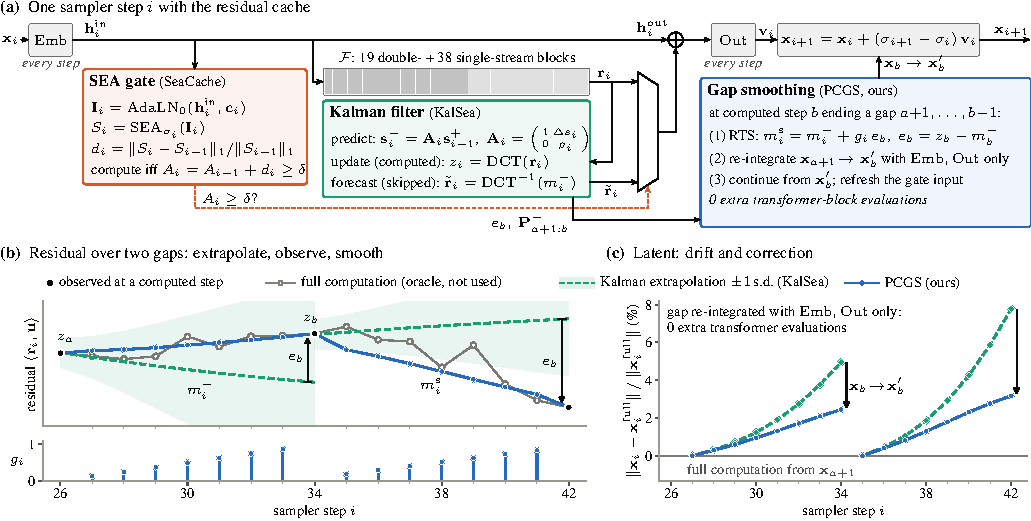
\includegraphics[width=\textwidth]{figures/method.pdf}
%     % Draft caption for the method figure (Fig. 2).  Usage in sections/method.tex:
%   \begin{figure*}[t]\centering
%     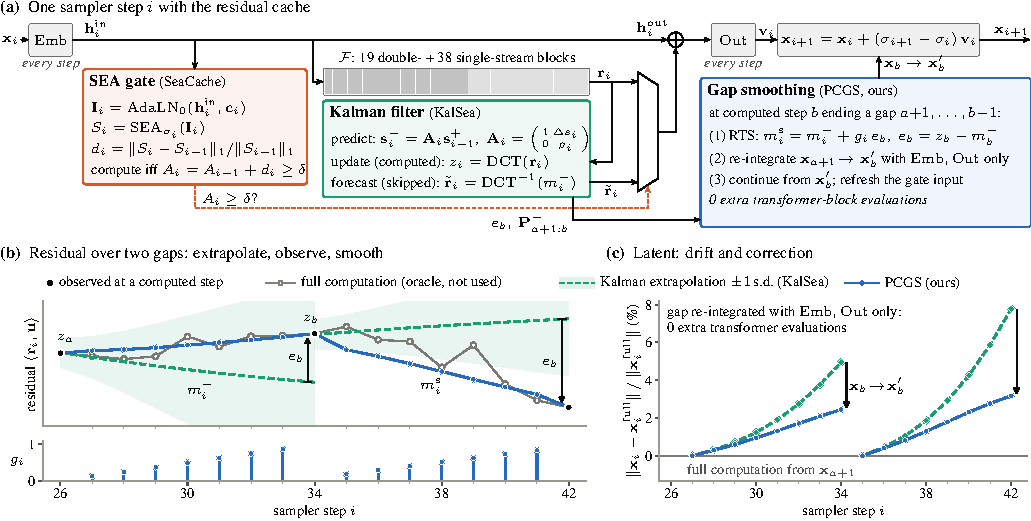
\includegraphics[width=\textwidth]{figures/method.pdf}
%     \input{figures/method_caption}
%   \end{figure*}
% Source and data: figures/src/method/ (build.sh).  Numbers below come from data/method_trace_summary.json
% (one real FLUX.1-dev generation, DrawBench prompt index 154, delta = 0.6, seed = 154).  Steps are 1-based (i = 1..N).
\caption{\textbf{Overview.}
\textbf{(a)}~In each sampler step~$i$, the \sea gate of \seacache accumulates the \sea-filtered relative $\ell_1$ change
$\gdist_i$ of the first block's modulated input and runs the transformer blocks $\blocks$ only when the accumulated change
reaches~$\delta$ (which resets it); the residual $\res_i=\blocks(\hin_i)-\hin_i$ of a computed step updates a damped-trend
Kalman filter per DCT coefficient (\kalsea), whose forecast $\resf_i$ replaces $\res_i$ on skipped steps, while $\Emb$
and $\Out$ run at every step.
\textbf{(b)}~When a computed step~$b$ ends the gap $a{+}1,\dots,b{-}1$, \pcgs propagates the innovation $e_b$ back into
the gap with the RTS gains $g_i$, which grow toward~$b$, so that the smoothed residuals $\smooth{m}_i$ replace the
extrapolation $\prior{m}_i$.
\textbf{(c)}~The gap is then re-integrated from $\lat_{a+1}$ with $\Emb$ and $\Out$ only and sampling continues from $\lat_b'$,
which roughly halves the latent deviation from full computation at~$b$ (here $5.0\%\to2.4\%$ and $7.8\%\to3.2\%$;
25--59\% lower in all ten gaps of this sample) at zero extra transformer evaluations.
Panels (b) and (c) show one real \flux generation at $\delta=0.6$ (13 of 50 steps computed) for the DrawBench prompt
whose PSNR gains (\kalsea over \seacache, \ours over \kalsea) are closest to the benchmark means (``McDonalds Church.'');
the residual is projected onto a fixed random unit direction~$\mathbf{u}$ in the lowest DCT band, which holds 89\% of the
residual energy, and the gray full-computation values come from extra evaluations made only for this figure.}
\label{fig:method}

%   \end{figure*}
% Source and data: figures/src/method/ (build.sh).  Numbers below come from data/method_trace_summary.json
% (one real FLUX.1-dev generation, DrawBench prompt index 154, delta = 0.6, seed = 154).  Steps are 1-based (i = 1..N).
\caption{\textbf{Overview.}
\textbf{(a)}~In each sampler step~$i$, the \sea gate of \seacache accumulates the \sea-filtered relative $\ell_1$ change
$\gdist_i$ of the first block's modulated input and runs the transformer blocks $\blocks$ only when the accumulated change
reaches~$\delta$ (which resets it); the residual $\res_i=\blocks(\hin_i)-\hin_i$ of a computed step updates a damped-trend
Kalman filter per DCT coefficient (\kalsea), whose forecast $\resf_i$ replaces $\res_i$ on skipped steps, while $\Emb$
and $\Out$ run at every step.
\textbf{(b)}~When a computed step~$b$ ends the gap $a{+}1,\dots,b{-}1$, \pcgs propagates the innovation $e_b$ back into
the gap with the RTS gains $g_i$, which grow toward~$b$, so that the smoothed residuals $\smooth{m}_i$ replace the
extrapolation $\prior{m}_i$.
\textbf{(c)}~The gap is then re-integrated from $\lat_{a+1}$ with $\Emb$ and $\Out$ only and sampling continues from $\lat_b'$,
which roughly halves the latent deviation from full computation at~$b$ (here $5.0\%\to2.4\%$ and $7.8\%\to3.2\%$;
25--59\% lower in all ten gaps of this sample) at zero extra transformer evaluations.
Panels (b) and (c) show one real \flux generation at $\delta=0.6$ (13 of 50 steps computed) for the DrawBench prompt
whose PSNR gains (\kalsea over \seacache, \ours over \kalsea) are closest to the benchmark means (``McDonalds Church.'');
the residual is projected onto a fixed random unit direction~$\mathbf{u}$ in the lowest DCT band, which holds 89\% of the
residual energy, and the gray full-computation values come from extra evaluations made only for this figure.}
\label{fig:method}
}{%
  \caption{\textbf{Overview of \ours.} \textbf{(a)}~One sampler step of a diffusion transformer with a residual cache.
    The input embedding $\Emb$ and the output layers $\Out$ run at every step. The \sea gate of
    \seacache~\cite{chung2026seacache} decides whether the block stack $\blocks$ runs. On computed steps the block-stack
    residual $\res_i$ updates a damped-trend Kalman filter; on skipped steps the filter's forecast replaces it.
    \textbf{(b)}~Predictor-corrector gap smoothing (\pcgs). When step $b$ is computed after the skipped steps
    $a{+}1,\dots,b{-}1$, the innovation $e_b$ (observed minus forecast residual) is distributed over the gap with the
    Rauch--Tung--Striebel smoother gains $g_i$, the gap is re-integrated with $\Emb$ and $\Out$ only, and sampling
    continues from the corrected latent $\lat'_b$. \pcgs adds no transformer evaluations.}
  \label{fig:method}}
\end{figure*}

\subsection{Preliminaries}
\label{sec:prelim}

\paragraph{Flow-matching sampling.}
Rectified-flow models~\cite{liu2023rectifiedflow,lipman2023flow,albergo2023interpolants,esser2024scaling} interpolate
$\lat_\sigma=(1-\sigma)\lat^\star+\sigma\boldsymbol\epsilon$ between data $\lat^\star$ and Gaussian noise
$\boldsymbol\epsilon$, and learn the velocity $\boldsymbol\epsilon-\lat^\star$. Sampling integrates the learned
velocity over a decreasing schedule $\sigma_0>\sigma_1>\dots>\sigma_N=0$ with Euler steps,
\begin{equation}
  \lat_{i+1}=\lat_i+(\sigma_{i+1}-\sigma_i)\,\vel_i,\qquad i=0,\dots,N-1.
  \label{eq:euler}
\end{equation}

\paragraph{Residual caching.}
A diffusion transformer computes the velocity in three stages,
\begin{equation}
  \hin_i=\Emb(\lat_i),\quad \hout_i=\blocks(\hin_i),\quad \vel_i=\Out(\hout_i,\cond_i),
  \label{eq:dit}
\end{equation}
where $\Emb$ embeds the latent patches, $\blocks$ is the block stack (in \flux, 19 double-stream and 38
single-stream blocks, which also process the text tokens), $\Out$ is the final adaptive normalization and linear
projection, and $\cond_i$ embeds the timestep and the guidance scale. Almost all computation is in $\blocks$.
Residual caches~\cite{liu2025teacache,chung2026seacache} store the block-stack residual of the image tokens,
$\res_i=\hout_i-\hin_i$, on computed steps. On skipped steps they run only $\Emb$ and $\Out$, with
$\hout_i=\hin_i+\hat\res_i$, where the filler $\hat\res_i$ is the last computed residual (reuse) or a forecast.

\paragraph{The \sea gate.}
TeaCache~\cite{liu2025teacache} and \seacache~\cite{chung2026seacache} decide whether to compute from the
timestep-modulated input of the first block, $\modin_i$, \ie, its adaptive layer normalization applied to $\hin_i$.
\seacache filters $\modin_i$ on the token grid with the normalized gain of the optimal linear denoiser under a
power-law spectrum, $G_i(f)\propto a_iS(f)/(a_i^2S(f)+b_i^2)$ with $S(f)=|f|^{-\beta}$, $a_i=1-\sigma_i$ and
$b_i=\sigma_i$, and accumulates the relative $\ell_1$ change of the filtered input,
\begin{equation}
  \gdist_i=\frac{\|\seaop_i(\modin_i)-\seaop_{i-1}(\modin_{i-1})\|_1}{\|\seaop_{i-1}(\modin_{i-1})\|_1},
  \quad D_i=D_{i-1}+\gdist_i.
  \label{eq:sea}
\end{equation}
Step $i$ is computed if $D_i\ge\delta$, after which $D_i$ is reset to zero, or if it is the first or the last step;
otherwise it is skipped. The threshold $\delta$ sets the budget. We use the official gate unchanged ($\beta=2$ for
images and 3 for videos).

\subsection{Kalman residual forecasting (predictor)}
\label{sec:kalman}

The residual evolves smoothly but nonlinearly along the trajectory, and the cache observes it only at the irregular
steps chosen by the gate. Following the state-space model of the contemporaneous SpecKCast~\cite{rajabi2026speckcast},
which forecasts the model output, we model every element of the residual as a damped trend observed in noise. The
state $\kstate_i=[m_i,\nu_i]^\top$ holds a value and its rate of change with respect to a time coordinate $s$ that
increases monotonically along the schedule, with steps $\ds_i=s(i)-s(i-1)$. At every step, computed or skipped, the
filter predicts
\begin{gather}
  \prior{\kstate}_i=\kA_i\,\post{\kstate}_{i-1},\qquad
  \prior{\kP}_i=\kA_i\,\post{\kP}_{i-1}\kA_i^\top+\kQ_i,\label{eq:predict}\\
  \kA_i=\begin{bmatrix}1&\ds_i\\0&\rho_i\end{bmatrix},\qquad
  \kQ_i=q\kappa\begin{bmatrix}\ds_i^3/3&\ds_i^2/2\\\ds_i^2/2&\ds_i\end{bmatrix},\nonumber
\end{gather}
with $\rho_i=e^{-\ds_i/\tau}$.
Here $\kQ_i$ is the process noise of an integrated Wiener process~\cite{barshalom2001estimation} with intensity $q\kappa$,
and $\rho_i$ damps the trend so that forecasts over long gaps do not overshoot~\cite{gardner1985forecasting}. On a
computed step $b$ the filter observes the residual element $z_b$ with noise variance $R$ and updates, with
$\mathbf h=[1,0]^\top$,
\begin{gather}
  e_b=z_b-\prior{m}_b,\quad S_b=[\prior{\kP}_b]_{00}+R,\quad \mathbf k_b=\prior{\kP}_b\mathbf h/S_b,\nonumber\\
  \post{\kstate}_b=\prior{\kstate}_b+\mathbf k_b\,e_b,\qquad
  \post{\kP}_b=(\mathbf I-\mathbf k_b\mathbf h^\top)\,\prior{\kP}_b.\label{eq:update}
\end{gather}
On skipped steps the moments are not updated ($\post{\kstate}_i=\prior{\kstate}_i$, $\post{\kP}_i=\prior{\kP}_i$),
and the cache writes the predicted value, $\hat\res_i=\prior{m}_i$, into $\hout_i=\hin_i+\hat\res_i$; the output
layers run as usual. The intensity $\kappa$ is adapted online so that the mean squared innovation matches its
predicted variance $S_b$~\cite{mehra1972approaches}: $\kappa\gets\mathrm{clip}_{[0.1,10]}(\kappa\,\gamma_b^{0.2})$,
where $\gamma_b$ is the ratio of the two, clipped to $[0.1,10]$.

\paragraph{Parametrizations.}
The covariance $\kP$ is shared by all elements (per-element variant) or by all coefficients of a frequency band (DCT
variant), so the filter costs a few elementwise operations per step and its gains are scalars per band. In the
\emph{per-element} variant, $s$ is a warped log signal-to-noise ratio of the schedule. In the
\emph{DCT} variant, which follows SpecKCast and is our default for \flux, the residual of each channel is transformed
with an orthonormal 2D DCT on the token grid, the coefficients are grouped into seven radial frequency bands, and each
band has its own warped time coordinate and covariance. Values are normalized by the residual power of their band.
The process-noise intensities, the initial trend variances and the band powers are calibrated once per model from 16
uncached trajectories whose prompts are disjoint from all evaluation prompts, and we use $\tau=0.5$ and $R=10^{-3}$
throughout (details in the supplement). The two variants perform the same (\cref{sec:ablations}). With the corrector of
\cref{sec:pcgs}, this predictor forms our full method, \ours; the predictor alone (the \sea gate with Kalman residual
forecasting) is labeled \kalsea in tables and figures.

\subsection{Predictor-corrector gap smoothing (corrector)}
\label{sec:pcgs}

Let $a<b$ be consecutive computed steps, so that $a{+}1,\dots,b{-}1$ is a gap of skipped steps. The predictor has
written $\hat\res_i=\prior{m}_i$ on the gap, and the sampler has advanced the latent from $\lat_{a+1}$ to $\lat_b$
with the corresponding velocities. At step $b$ the block stack runs and the filter observes $z_b$. The innovation
$e_b$ is the forecast error at the end of the gap; the forecast errors inside the gap are correlated with it, since
they stem from the same trend error and process noise. \pcgs exploits this correlation in four steps.

\paragraph{(1) Smoothing.}
No observation falls inside the gap, so $\kstate_b=\kPhi(b,i)\,\kstate_i+\mathbf w_{i\to b}$ for $a<i<b$, with the
transition $\kPhi(b,i)=\kA_b\kA_{b-1}\cdots\kA_{i+1}$ and accumulated process noise $\mathbf w_{i\to b}$ independent
of $\kstate_i$. Given the observations up to step $a$, the cross-covariance of $\kstate_i$ and $z_b$ is therefore
$\prior{\kP}_i\kPhi(b,i)^\top\mathbf h$, and conditioning the joint Gaussian on $z_b$ yields
\begin{equation}
  \smooth{m}_i=\prior{m}_i+g_i\,e_b,\qquad
  g_i=\frac{\big[\prior{\kP}_i\,\kPhi(b,i)^\top\big]_{00}}{[\prior{\kP}_b]_{00}+R}.
  \label{eq:smooth}
\end{equation}
This is the RTS smoother~\cite{rauch1965maximum} over $[a,b]$: inside the gap the filtered and predicted moments
coincide, so the products of the smoother gains $\post{\kP}_i\kA_{i+1}^\top(\prior{\kP}_{i+1})^{-1}$ telescope into
$\prior{\kP}_i\kPhi(b,i)^\top(\prior{\kP}_b)^{-1}$ (proof in the supplement). The gains use only quantities that the
filter already maintains, so the smoother has no parameters of its own. They increase across the gap: the steps
closest to $b$, whose forecasts were the least reliable, absorb most of the innovation. In residual space, the smoothed
residual is the forecast plus a gain-weighted share of the forecast error revealed at $b$,
\begin{equation}
  \resf_i=\hat\res_i+\mathcal G_i\big(\res_b-\hat\res_b\big),\qquad a<i<b,
  \label{eq:smooth-res}
\end{equation}
where $\hat\res_b=\prior{m}_b$ is the forecast for step $b$, and $\mathcal G_i$ multiplies by the scalar $g_i$
(per-element variant) or applies the band gains $g_{i,\ell}$ in the DCT domain.

\paragraph{(2) Re-integration.}
Only the output layers depend on the residual. We therefore replay the sampler over the gap with the smoothed
residuals, starting from the latent that the sampler actually used at the first skipped step, $\lat'_{a+1}=\lat_{a+1}$;
for $a<i<b$,
\begin{equation}
  \lat'_{i+1}=\lat'_i+(\sigma_{i+1}-\sigma_i)\,\Out\big(\Emb(\lat'_i)+\resf_i,\cond_i\big).
  \label{eq:reint}
\end{equation}
Re-embedding the corrected latents $\lat'_i$, instead of reusing the stored inputs $\hin_i$, makes the replay an exact
Euler integration with the smoothed residuals; a batched variant that reuses $\hin_i$ is ablated in
\cref{sec:ablations}.

\paragraph{(3) Continuation.}
The block stack at step $b$ was evaluated on the uncorrected latent $\lat_b$. Instead of evaluating it again, we keep
its residual $\res_b$, attach it to the corrected input, and absorb the latent correction into the velocity returned
to the sampler:
\begin{equation}
  \vel'_b=\Out\big(\Emb(\lat'_b)+\res_b,\cond_b\big)+\frac{\lat'_b-\lat_b}{\sigma_{b+1}-\sigma_b}.
  \label{eq:offset}
\end{equation}
The unmodified Euler step~\eqref{eq:euler} then produces
$\lat_{b+1}=\lat'_b+(\sigma_{b+1}-\sigma_b)\,\Out(\Emb(\lat'_b)+\res_b,\cond_b)$, \ie, sampling continues from
$\lat'_b$, and \pcgs remains a drop-in replacement of the network output.

\paragraph{(4) Gate refresh.}
We recompute the gate's reference input of step $b$ from $\lat'_b$ (one adaptive normalization and one \sea filter),
so that the gate follows the corrected trajectory; this detail has no measurable effect (\cref{sec:ablations}).

\paragraph{Why smoothing corrects the latent.}
To first order, the latent error at step $b$ is a linear function of the residual errors in the gap, each scaled by
its step size and propagated by Jacobians of $\Emb$ and $\Out$. Substituting conditional means into a linear function
minimizes its expected squared error, so, under the filter's model and to first order, re-integrating with the
smoothed residuals minimizes the expected squared error of $\lat'_b$ given the observations up to step $b$; the
forecasts are optimal only given those up to step $a$.

\paragraph{Remarks.}
\pcgs does not change the predictor for the next gap, because smoothed and filtered estimates coincide at the latest
observation. It only requires the solver update to be linear in the network output: for a multistep solver such as
the UniPC sampler~\cite{zhao2023unipc} of Wan2.1, the solver state is restored at step $a{+}1$ and the updates are
replayed with the corrected outputs; with classifier-free guidance~\cite{ho2022cfg}, the conditional and
unconditional residuals are filtered and smoothed separately under a shared gate. For plain reuse, the smoother of the
corresponding random-walk model with noise-free observations is the linear interpolation between $\res_a$ and
$\res_b$. \cref{alg:kalsea} summarizes the procedure.

% Requires \usepackage{algorithm} and \usepackage{algpseudocode} (added to macros.tex).
\begin{algorithm}[t]
  \caption{\ours sampling. The second \textbf{if} block is \pcgs; without it, the procedure is the predictor
  alone (\kalsea).}
  \label{alg:kalsea}
  \small
  \begin{algorithmic}[1]
    \Require noise $\lat_0$, schedule $\sigma_0>\dots>\sigma_N=0$, threshold $\delta$
    \State $D\gets0$;\; gap $\mathcal S\gets\emptyset$
    \For{$i=0,\dots,N-1$}
      \State $\hin_i\gets\Emb(\lat_i)$;\; $D\gets D+\gdist_i$;\; predict \Comment{\eqref{eq:sea},\,\eqref{eq:predict}}
      \If{$i\in\{0,N-1\}$ \textbf{or} $D\ge\delta$} \Comment{computed step, $b=i$}
        \State $\res_i\gets\blocks(\hin_i)-\hin_i$;\; $D\gets0$;\; Kalman update \Comment{\eqref{eq:update}}
        \State $\vel_i\gets\Out(\hin_i+\res_i,\cond_i)$
      \Else \Comment{skipped step}
        \State $\hat\res_i\gets\prior{m}_i$;\; $\vel_i\gets\Out(\hin_i+\hat\res_i,\cond_i)$;\; $\mathcal S\gets\mathcal S\cup\{i\}$
      \EndIf
      \If{step $i$ was computed \textbf{and} $\mathcal S\neq\emptyset$}
        \State $\resf_j\gets\hat\res_j+\mathcal G_j(\res_i-\hat\res_i)$, $j\in\mathcal S$ \Comment{\eqref{eq:smooth-res}}
        \State $\lat'\gets\lat_{\min\mathcal S}$ \Comment{\eqref{eq:reint}}
        \For{$j\in\mathcal S$ in ascending order}
          \State $\lat'\gets\lat'+(\sigma_{j+1}-\sigma_j)\,\Out(\Emb(\lat')+\resf_j,\cond_j)$
        \EndFor
        \State $\vel_i\gets\Out(\Emb(\lat')+\res_i,\cond_i)+\frac{\lat'-\lat_i}{\sigma_{i+1}-\sigma_i}$ \Comment{\eqref{eq:offset}}
        \State recompute the gate reference from $\lat'$;\; $\mathcal S\gets\emptyset$
      \EndIf
      \State $\lat_{i+1}\gets\lat_i+(\sigma_{i+1}-\sigma_i)\,\vel_i$ \Comment{unchanged sampler}
    \EndFor
    \State \Return $\lat_N$
  \end{algorithmic}
\end{algorithm}

\subsection{Cost}
\label{sec:cost}

\ours performs exactly the block-stack evaluations of the gate's schedule; \pcgs adds none. It adds one evaluation of
$\Emb$ and $\Out$ per skipped step and, at each computed step that closes a gap, one more of each plus the gate
refresh. For \flux at $1024^2$, $\Emb$ and $\Out$ are linear maps between 64 and 3072 channels over 4096 tokens,
about 3.4\,GFLOP per skipped step, whereas one transformer evaluation costs 59.5\,TFLOPs (2976 for 50
steps~\cite{chung2026seacache}); over an image, \pcgs costs about 0.3\% of one transformer evaluation. The filter
state and the gap buffer raise the peak memory by 0.16\,GiB over the uncached sampler (\seacache: 0.05\,GiB;
\kalsea: 0.14\,GiB).
% Wall-clock overhead: to be added with the controlled latency measurement (latency columns are blank until then).
% FLOP count (analytic, from the layer shapes; verify with calflops before submission): x_embedder Linear(64->3072)
% and proj_out Linear(3072->64) on 4096 tokens cost 2*4096*64*3072 = 1.61 GFLOP each, norm_out ~0.1 GFLOP, i.e.
% ~3.36 GFLOP per skipped step. Per image at delta 0.6: 37 skipped steps + 10 corrected computed steps (+ gate refresh,
% ~1.7 GFLOP each, mostly the 2D FFTs of the SEA filter) ~ 0.18 TFLOP = 0.29% of 59.5 TFLOPs; delta 0.3: ~0.28%.
% Memory: eval2 dMem = mean peak allocated memory minus that of the 50-step reference (33.85 GiB), DrawBench-200.

\section{Experiments}
\label{sec:experiments}

% Number sources (all FLUX.1-dev, DrawBench-200, eval2 paired bootstrap, 10k resamples, seed 0):
%   research_v2/runs/drawbench_eval/eval_two_budgets_vs_seacache.txt, eval_sweep_vs_seacache.txt,
%   eval_sweep_vs_kalsea.txt, eval_final.txt, eval_dct_pcgs.txt, eval_pairs2.txt; linear extrapolation =
%   runs/drawbench/linext_<d> (generic first-order extrapolation, metrics_sweep/main.json), paired
%   bootstrap recomputed with the eval2 procedure. Correction sizes: plugin_stats (dx_rel, gap_len) in the stats files of
%   research_v2/runs/drawbench/kalsea_dct_pcgs_<d>.

\subsection{Setup}
\label{sec:setup}

\paragraph{Models and protocol.}
We follow the protocol of \seacache~\cite{chung2026seacache}. For text-to-image generation we use
\flux~\cite{blackforestlabs2024flux} at $1024{\times}1024$ with 50 Euler steps of its default flow-matching schedule,
embedded guidance 3.5, and the 200 DrawBench prompts~\cite{saharia2022imagen}; the seed of each image is its prompt
index and is shared by all methods. For text-to-video generation we use HunyuanVideo~\cite{kong2024hunyuanvideo} at
$480{\times}640$ with 65 frames and Wan2.1-T2V-1.3B~\cite{wan2025wan} at $832{\times}480$ with 81 frames, both with 50
steps, on the 944 unique VBench prompts~\cite{huang2024vbench}. \TODO{Video seeds.} Each accelerated sample is compared
with the output of the uncached 50-step sampler for the same prompt and seed.

\paragraph{Budgets and baselines.}
All caches use the official \sea gate, and the budget is set by its threshold $\delta$. We report the mean number of
block-stack evaluations per image (\nfe, out of 50), counted by hooks on every block. Since the gate is closed-loop and
\pcgs refreshes its reference, different fillers can produce slightly different schedules; we only compare at matched
\nfe. On \flux, $\delta=0.3$ and $0.6$ give 20.8 and 13.0 \nfe, and at $\delta=0.6$ our run of \seacache reproduces its
published PSNR (21.26 vs.\ 21.33\,dB~\cite{chung2026seacache}). At these two thresholds \seacache, \kalsea and \ours
computed exactly the same steps for 188 and 182 of the 200 prompts, and the per-prompt \nfe never differs by more than
one, so the comparison isolates what is written on skipped steps. Behind the same gate we compare four fillers: reuse of
the last residual (\seacache), linear extrapolation of the residual from the last two computed steps (the first-order
finite-difference forecast of TaylorSeer~\cite{liu2025taylorseer}), the Kalman forecast (\kalsea), and the Kalman
forecast with \pcgs (\ours). \TODO{Rows for TeaCache, TaylorSeer, $\Delta$-DiT and ToCa at matched budgets, if run.}

\paragraph{Metrics.}
We report PSNR on 8-bit RGB, SSIM~\cite{wang2004ssim} (scikit-image, $7{\times}7$ window) and LPIPS with AlexNet
features~\cite{zhang2018lpips}, each against the 50-step reference and averaged over prompts. For differences between
methods we report paired bootstrap 95\% confidence intervals over prompts (10{,}000 resamples, percentile intervals)
and the fraction of prompts on which a method is better. \TODO{TFLOPs (counted as in \seacache) and latency, measured
for all methods under identical conditions; until then the tables show \nodata.}

\paragraph{Development and test prompts.}
All design decisions (the smoother, the re-integration and continuation rules, $\tau$ and $R$) were made on a
development set of 64 COCO captions~\cite{lin2014coco}, and the forecaster was calibrated on 16 other COCO captions.
DrawBench was only used to score finished configurations and is thus a held-out test set. Development-set results are
reported in the supplement.

\paragraph{Implementation.}
\ours replaces the forward pass of the transformer in diffusers; the scheduler is unchanged, and the re-integration
\eqref{eq:reint} reproduces its arithmetic. All runs use bf16 on NVIDIA B200 GPUs. For video we use the per-element
filter, since the DCT bands are defined on 2D token grids. \TODO{Video implementation details (calibration, UniPC
replay for Wan2.1).}

\maybeinput{tables/tab_flux_main}

\subsection{Comparison at matched \nfe}
\label{sec:main-results}

\cref{tab:flux-main} compares the fillers at the two budgets of the protocol. At 20.8 \nfe, \ours improves over
\seacache by 2.73\,dB PSNR (95\% CI [2.34, 3.12]; better on 88\% of the prompts), 0.031 SSIM [0.027, 0.036] and
0.033 LPIPS [0.029, 0.037]. At 13 \nfe the gains are 1.27\,dB [1.02, 1.52] (79\% of the prompts), 0.042 SSIM
[0.035, 0.048] and 0.060 LPIPS [0.052, 0.068]. Forecasting explains part of this improvement, as both forecasters
improve over reuse: linear extrapolation reaches 28.51 and 21.80\,dB and \kalsea 28.79 and 21.91\,dB at the two budgets.
\pcgs adds 0.83\,dB [0.63, 1.02] at 20.8 \nfe and 0.61\,dB [0.48, 0.76] at 13 \nfe on top of \kalsea, with better PSNR
on 81\% and 78\% of the prompts, and \ours exceeds linear extrapolation by 1.11\,dB [0.89, 1.34] and 0.73\,dB
[0.54, 0.92]. The median per-prompt gain of \pcgs over \kalsea is 0.60 and 0.44\,dB; on the remaining 19\% and 22\% of
the prompts it lowers PSNR, by at most 3.6 and 2.3\,dB.
% Linear extrapolation is not in tab_flux_main (generated by figures/src/make_tables.py); NFE 20.84 / 13.00, SSIM
% 0.925 / 0.827, LPIPS 0.061 / 0.171. Suggest adding it as a row "Lin. extrapolation" (generic baseline).

\begin{figure*}[t]
  \centering
  \maybegraphics[width=\textwidth]{figures/fig_tradeoff.pdf}
  \IfFileExists{figures/fig_tradeoff_caption.tex}{% Auto-generated by figures/src/make_captions.py (numbers from figures/src/data). Usage:
% \begin{figure*}[t]\centering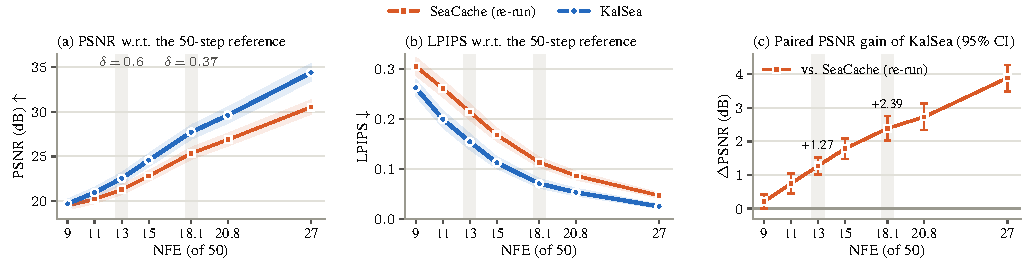
\includegraphics[width=\textwidth]{figures/fig_tradeoff.pdf}% Auto-generated by figures/src/make_captions.py (numbers from figures/src/data). Usage:
% \begin{figure*}[t]\centering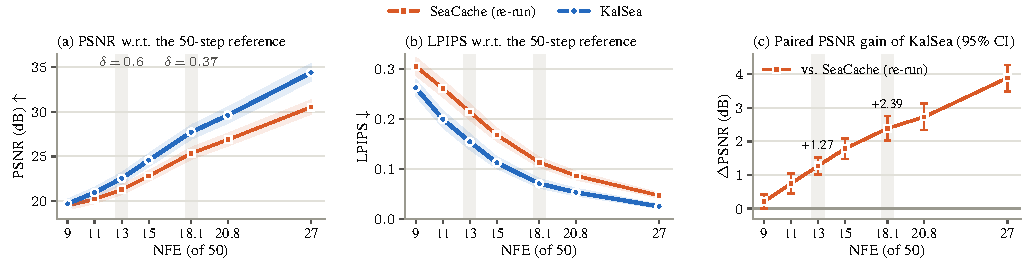
\includegraphics[width=\textwidth]{figures/fig_tradeoff.pdf}\input{figures/fig_tradeoff_caption}\end{figure*}   (one-column variant: figures/fig_tradeoff_1col.pdf, width=\columnwidth, same caption)
\caption{\textbf{Quality--compute trade-off on \flux} (DrawBench, 200 held-out prompts). \textbf{(a)}~PSNR and \textbf{(b)}~LPIPS with respect to the 50-step reference vs.\ the mean number of transformer evaluations per image (\nfe). The budget is set by the \sea-gate threshold $\delta \in \{0.2, 0.3, 0.37, 0.5, 0.6, 0.8, 1.0\}$, shared by all methods; gray bands mark the two budgets of \cref{tab:flux-main} ($\delta = 0.3$, $0.6$). Lines: means over prompts; shaded: 95\% bootstrap CIs. \textbf{(c)}~Paired per-prompt PSNR gain of \ours over \seacache and over \kalsea (mean, 95\% bootstrap CI). The gain over \seacache grows with the budget, from +0.21\,dB [$-$0.005, +0.42] at 9 \nfe (not significant; LPIPS still improves by 0.043 [0.033, 0.053]) to +3.89\,dB [+3.49, +4.28] at 27 \nfe; the gain over \kalsea (gap smoothing alone) is positive at every budget. \seacache: \sea gate with residual reuse; \kalsea: \sea gate with Kalman residual forecasting; \ours: \kalsea with predictor-corrector gap smoothing.}
\label{fig:tradeoff}
\end{figure*}   (one-column variant: figures/fig_tradeoff_1col.pdf, width=\columnwidth, same caption)
\caption{\textbf{Quality--compute trade-off on \flux} (DrawBench, 200 held-out prompts). \textbf{(a)}~PSNR and \textbf{(b)}~LPIPS with respect to the 50-step reference vs.\ the mean number of transformer evaluations per image (\nfe). The budget is set by the \sea-gate threshold $\delta \in \{0.2, 0.3, 0.37, 0.5, 0.6, 0.8, 1.0\}$, shared by all methods; gray bands mark the two budgets of \cref{tab:flux-main} ($\delta = 0.3$, $0.6$). Lines: means over prompts; shaded: 95\% bootstrap CIs. \textbf{(c)}~Paired per-prompt PSNR gain of \ours over \seacache and over \kalsea (mean, 95\% bootstrap CI). The gain over \seacache grows with the budget, from +0.21\,dB [$-$0.005, +0.42] at 9 \nfe (not significant; LPIPS still improves by 0.043 [0.033, 0.053]) to +3.89\,dB [+3.49, +4.28] at 27 \nfe; the gain over \kalsea (gap smoothing alone) is positive at every budget. \seacache: \sea gate with residual reuse; \kalsea: \sea gate with Kalman residual forecasting; \ours: \kalsea with predictor-corrector gap smoothing.}
\label{fig:tradeoff}
}{%
  \caption{\textbf{Fidelity versus compute on \flux} (DrawBench, 200 held-out prompts). The \sea-gate threshold
    $\delta\in\{1.0, 0.8, 0.6, 0.5, 0.37, 0.3, 0.2\}$ sets the budget (9 to 27 of 50 transformer evaluations); all
    methods share the gate and are compared at matched \nfe. \textbf{(a)}~PSNR and \textbf{(b)}~LPIPS with respect to
    the 50-step sampler; shaded bands are 95\% bootstrap confidence intervals of the mean. \textbf{(c)}~Paired PSNR gain
    of \ours over \seacache and over \kalsea, with 95\% confidence intervals. Gray columns mark the two budgets of
    \cref{tab:flux-main}; all numbers are listed in the supplement.}
  \label{fig:tradeoff}}
\end{figure*}

\paragraph{Budget sweep.}
\cref{fig:tradeoff} varies $\delta$ from 0.2 to 1.0 (27 to 9 \nfe). \ours attains the highest PSNR and the lowest LPIPS
at every budget. Its PSNR gain over \seacache grows with the budget, from 0.74\,dB [0.46, 1.04] at 11 \nfe to 3.89\,dB
[3.49, 4.28] at 27 \nfe; at 9 \nfe the PSNR gain is not significant (0.21\,dB [$-$0.005, 0.42]), whereas LPIPS still
improves by 0.043 [0.033, 0.053]. The predictor alone behaves as the open-loop argument of \cref{sec:intro} predicts:
the gain of \kalsea over reuse shrinks from 2.37\,dB at 27 \nfe to 0.11\,dB [$-$0.14, 0.34] at 11 and $-$0.10\,dB
[$-$0.31, 0.10] at 9 \nfe, and linear extrapolation even falls below reuse at 11 and 9 \nfe ($-$0.58 and $-$0.77\,dB),
because forecast errors accumulate over the long gaps of small budgets. \pcgs improves on \kalsea at every budget, by
0.31\,dB [0.24, 0.39] at 9 \nfe and up to 1.52\,dB [1.30, 1.75] at 27 \nfe.

\paragraph{Size of the correction.}
The relative latent correction $\|\lat'_b-\lat_b\|/\|\lat_b\|$ grows with the length of the gap. At 13 \nfe it
averages 0.7\% after single skipped steps and 4.1\% after the seven-step gaps, which contain a third of all skipped
steps (2.0\% over all gaps); at 20.8 \nfe, where most skipped steps lie in three-step gaps, it averages 0.7\%.

\begin{figure*}[t]
  \centering
  \maybegraphics[width=\textwidth]{figures/fig_qualitative.pdf}
  \IfFileExists{figures/fig_qualitative_caption.tex}{% Auto-generated by figures/src/make_captions.py (numbers from figures/src/data). Usage:
% \begin{figure*}[t]\centering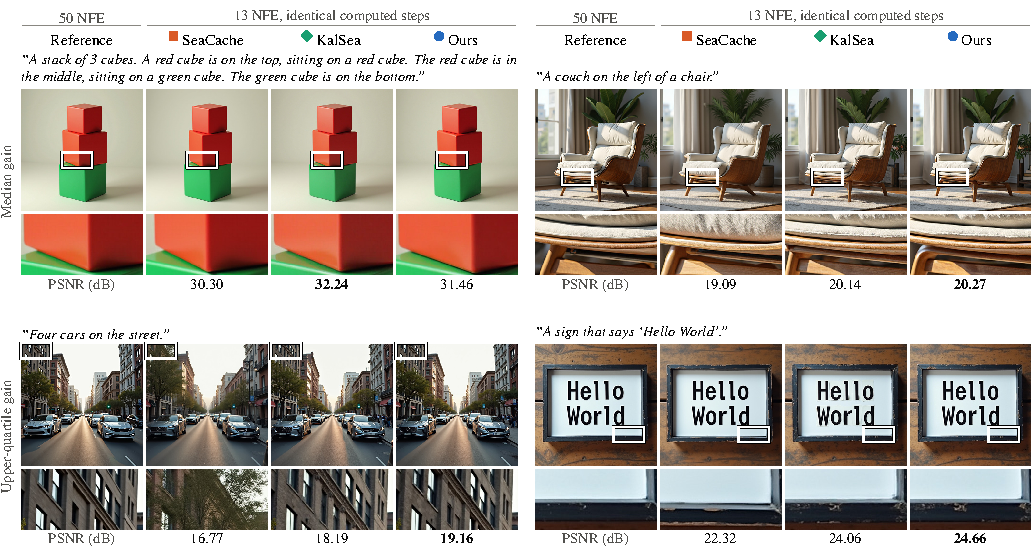
\includegraphics[width=\textwidth]{figures/fig_qualitative.pdf}% Auto-generated by figures/src/make_captions.py (numbers from figures/src/data). Usage:
% \begin{figure*}[t]\centering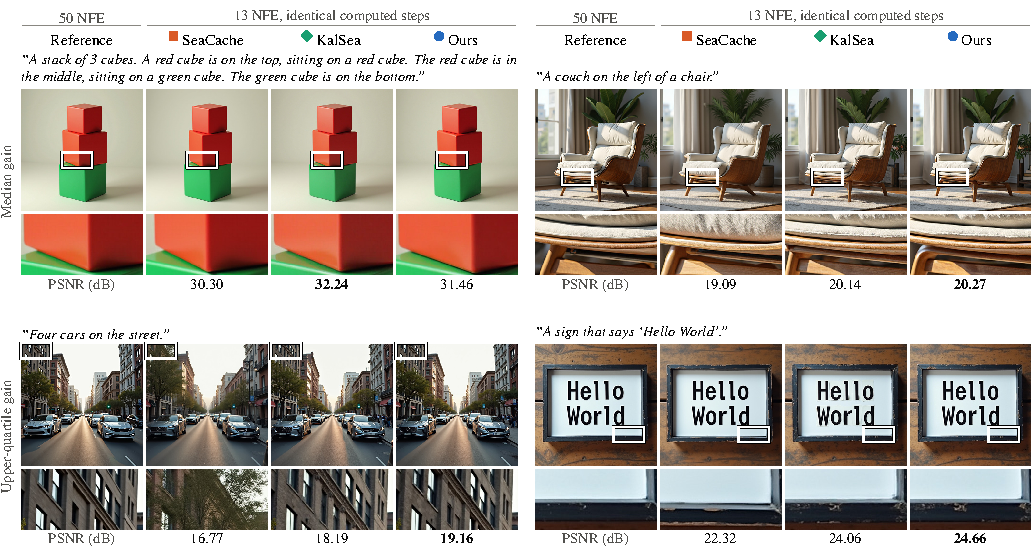
\includegraphics[width=\textwidth]{figures/fig_qualitative.pdf}\input{figures/fig_qualitative_caption}\end{figure*}
\caption{\textbf{Qualitative comparison at 13 \nfe} (\flux, DrawBench, $\delta = 0.6$, $3.8\times$ fewer transformer evaluations than the 50-step reference). The prompts are selected by a fixed rule, not by hand: among the 188 of 200 prompts on which \seacache and \ours computed the identical set of steps, we compute the per-prompt PSNR gain of \ours over \seacache and show the two prompts whose gain is closest to the median (+1.19\,dB; top row) and the two closest to the upper quartile (+2.40\,dB; bottom row). Below each image, a fixed $256\times128$-pixel crop (of $1024\times1024$) is magnified; it is placed where the two accelerated samples differ most (largest mean absolute difference), without looking at the reference. Numbers: PSNR (dB) with respect to the reference, best in bold. Examples near the lower quartile and at the $\approx$21-\nfe budget are in the supplementary material.}
\label{fig:qualitative}
\end{figure*}
\caption{\textbf{Qualitative comparison at 13 \nfe} (\flux, DrawBench, $\delta = 0.6$, $3.8\times$ fewer transformer evaluations than the 50-step reference). The prompts are selected by a fixed rule, not by hand: among the 188 of 200 prompts on which \seacache and \ours computed the identical set of steps, we compute the per-prompt PSNR gain of \ours over \seacache and show the two prompts whose gain is closest to the median (+1.19\,dB; top row) and the two closest to the upper quartile (+2.40\,dB; bottom row). Below each image, a fixed $256\times128$-pixel crop (of $1024\times1024$) is magnified; it is placed where the two accelerated samples differ most (largest mean absolute difference), without looking at the reference. Numbers: PSNR (dB) with respect to the reference, best in bold. Examples near the lower quartile and at the $\approx$21-\nfe budget are in the supplementary material.}
\label{fig:qualitative}
}{%
  \caption{\textbf{Qualitative comparison on \flux at 13 \nfe} (held-out DrawBench prompts). For these prompts the
    three caches computed the same steps. Prompts are chosen by a fixed rule: among the prompts with identical
    schedules, those whose PSNR gain of \ours over \seacache is closest to the median (top) and to the upper quartile
    (bottom). Zoom windows are placed where the three cached images differ most from each other, without using the
    reference. Numbers: PSNR with respect to the 50-step sampler.}
  \label{fig:qualitative}}
\end{figure*}

\paragraph{Qualitative results.}
\cref{fig:qualitative} shows prompts selected by a fixed rule rather than by hand. With the same computed steps, reuse
blurs or alters high-frequency structure such as facades and upholstery, the Kalman forecast recovers part of it, and
\pcgs brings the details closer to the reference. The improvement is not uniform: on some prompts the predictor alone
is already as close to the reference as \ours. \TODO{Sync with the final figure; more examples at 13 and 20.8 \nfe in
the supplement.}

\subsection{Video generation}
\label{sec:video}

\maybeinput{tables/tab_video_main}

We apply \ours with the per-element filter to HunyuanVideo and Wan2.1-1.3B at the two thresholds of \seacache
(HunyuanVideo: $\delta=0.19$ and 0.35; Wan2.1: $\delta=0.2$ and 0.35). HunyuanVideo samples with Euler steps and a
single guidance-distilled branch, so \pcgs applies exactly as in \cref{sec:pcgs}; Wan2.1 uses UniPC with
classifier-free guidance and requires the solver replay described there. \cref{tab:video-main} reports the results.
\TODO{Results and discussion; VBench scores in the supplement.}

\subsection{Ablations}
\label{sec:ablations}

\maybeinput{tables/tab_ablation_2x2}

\paragraph{Forecaster parametrization.}
\cref{tab:ablation-2x2} crosses the two parametrizations of the predictor with \pcgs. \pcgs improves both by similar
amounts: by 0.78\,dB [0.60, 0.97] and 0.61\,dB [0.48, 0.75] with DCT bands, and by 0.83\,dB [0.66, 1.01] and 0.58\,dB
[0.44, 0.73] per element, at 18.1 and 13 \nfe. With \pcgs, the two parametrizations differ by 0.02\,dB [$-$0.09, 0.15]
and 0.01\,dB [$-$0.13, 0.15]. Unlike for forecasting the model output~\cite{rajabi2026speckcast}, the frequency
decomposition is unnecessary for the residual, and the simpler per-element filter suffices; we use it for video.
% The DCT rows without PCGS in tab_ablation_2x2 are the same-harness rerun of KalSea (kalsea_main_<d>), which differs
% from the KalSea run in tab_flux_main / fig_tradeoff (speckcast_<d>) by +0.03 / +0.00 dB.

\maybeinput{tables/tab_ablation_main}

\paragraph{Anatomy of the corrector.}
\cref{tab:ablation} isolates the parts of \pcgs on DrawBench at 20.8 and 13 \nfe. \TODO{Numbers from the generated
ablation table once the runs are scored; report each row as a paired difference to \ours.}
% Table: tables/tab_ablation_main.tex, generated by research_v2/ablations/make_tables.py with \label{tab:ablation}.
The rows compare: correcting only the filter state, without re-integrating
the latent (\tbd); re-integration with a linear interpolation from $\res_a$ to $\res_b$ that ignores the forecast
(\tbd), with the forecast plus a linearly weighted innovation (\tbd), with a quadratic interpolation through the last
three computed residuals (\tbd), and with the RTS gains (\ours); a batched re-integration that reuses the stored inputs
$\hin_i$ instead of re-embedding the corrected latents (\tbd); and \pcgs without the gate refresh (\tbd). On the
development set, the exact re-integration was better than the batched one by 0.36\,dB at 18 \nfe (0.10\,dB at 13 \nfe,
not significant), the linear interpolation performed similarly to the RTS gains (difference $-$0.13 and $+$0.07\,dB,
both intervals include zero), and the gate refresh had no measurable effect (supplement).
% Development-set numbers: research_v2/ablations/ABLATIONS_devset.md (COCO-64, n = 62-64, per-element forecaster).

\paragraph{Other fillers and forecaster settings.}
The correction is not tied to the Kalman forecaster. With reuse, the corresponding smoother interpolates linearly
between $\res_a$ and $\res_b$; on the development set this improves reuse by 1.31\,dB [1.00, 1.59] and 0.77\,dB
[0.57, 0.97] at 18 and 13 \nfe. \TODO{DrawBench rows: reuse + \pcgs and linear extrapolation + \pcgs (\tbd).} We also
test the trend damping $\tau=0.1$ used by SpecKCast (\tbd). With a calibration-free per-element filter, \pcgs still
adds 0.83 and 0.51\,dB on the development set. Forecasting a quantity of the sampler instead of the residual (the
clean-image, noise or velocity prediction reconstructed from the current latent) was not better on the development
set (supplement).

\paragraph{Noise floor.}
The band statistics of the filter are accumulated with atomic GPU additions, so two runs of the same configuration are
not bitwise identical. Two runs of \kalsea differ by 0.03\,dB [$-$0.003, 0.067] at 18.1 \nfe and by 0.002\,dB
[$-$0.008, 0.011] at 13 \nfe in mean PSNR; we make no claims about differences below 0.1\,dB.

\section{Conclusion}
\label{sec:conclusion}

Caches for diffusion transformers decide when to skip the block stack and what to write instead, but the fillers they
use are open loop: the errors of skipped steps are integrated into the latent and never corrected. \pcgs closes this
loop at no cost in network evaluations. It treats each skipped gap as a smoothing problem, estimates the residuals of
the gap with the RTS smoother of the forecaster's own state-space model once the next step is computed, and
re-integrates the gap through the output layers. Combined with the \sea gate and a Kalman residual forecaster, it
improves fidelity to the 50-step sampler at every budget we tested on \flux, with gains over reuse that grow with the
budget. \TODO{One sentence on video.} Promising directions are to choose the computed steps jointly with the
corrector, rather than with a gate designed for reuse, and to apply the correction to caches that operate on features
inside the block stack.

\paragraph{Limitations.}
Matched \nfe is not matched latency: \pcgs adds output-layer evaluations (about 0.3\% of one transformer evaluation per
image) and 0.02\,GiB of memory over \kalsea, and the filter adds elementwise work on every step.
\TODO{Latency once measured.} Our metrics measure fidelity to the 50-step sampler, which is the goal of a cache but
not the same as sample quality. The filter's band statistics are accumulated with atomic GPU additions, so runs are not
bitwise reproducible (0.03\,dB between two runs of the same configuration). All design decisions were made on a
development set of COCO captions and evaluated on held-out DrawBench prompts, but our image results cover a single
model. At a computed step, \pcgs attaches the residual evaluated at the uncorrected latent to the corrected one, an
approximation that is accurate only for small corrections; at the smallest budget, with gaps of up to twelve steps, its
gain is modest (0.31\,dB at 9 \nfe).
\unskip
\label{endofbody}\par% records the page where the body ends (page-limit check in tools/pdfcheck.py); the \par keeps
% the spaces of the bibliography block below from adding an empty last line to the conclusion.
% Mandatory for CVPR 2027 (Author Guidelines): placed after the main text and before the references; does not count
% toward the 8-page limit; must not reveal the authors' identities. A missing statement leads to desk rejection.
% DRAFT wording, to be confirmed by the authors: it must describe the actual use of LLM tools accurately.
\section*{LLM Usage Statement}
LLM-based assistants were used in this work to propose and implement method variants and experiment code, to run and
monitor experiments and evaluation scripts, to draft and edit text and figures, and to check the reported numbers
against the logged results. The authors directed the research and take full responsibility for the content of this
paper.
% mandatory for CVPR 2027: after the main text, before the references (extra page)
{
    \small
    \bibliographystyle{ieeenat_fullname}
    \bibliography{refs}
}

% Supplementary material is a separate PDF (due Mon Nov 23, 2026 AoE): supp_main.tex -> supp.pdf (built by build.sh
% after this file; it imports the labels of build/main.aux). Do not append it here.

\end{document}
